% ==========================================================================================================================
\section{Operaciones SNMP}
% ==========================================================================================================================

% ==========================================================================================================================
\subsection{Ejercicio MIB}
% ==========================================================================================================================

\noindent
Para demostrar las consultas SNMP y la forma para acceder a los objetos de la MIB se realizan las siguientes consultas.

\noindent
\newline
\textbf{consulta 1:} ¿Cuándo fue el último reinicio (Dia, hora y minuto) de los agentes?

\begin{figure}[htbp!]
	\centering
		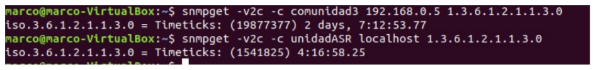
\includegraphics[width=0.8\textwidth]{images/capturas/pregunta1}
	\caption{Consulta SNMP1.}
\end{figure}

\textbf{consulta 2:} ¿Cuántas interfaces Ethernet tienen?

\begin{figure}[htbp!]
	\centering
		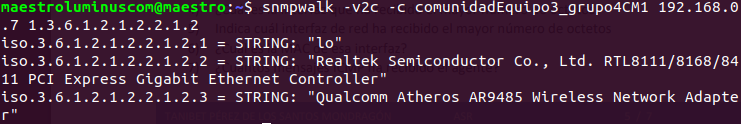
\includegraphics[width=0.8\textwidth]{images/capturas/pregunta2}
	\caption{Consulta SNMP2.}
\end{figure}

\textbf{consulta 3:} ¿Cuál es la velocidad (en MBPS) de esas interfaces?
\begin{figure}[htbp!]
	\centering
		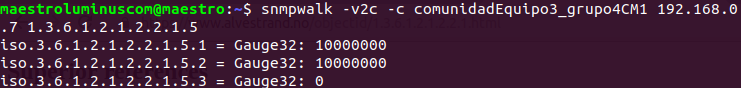
\includegraphics[width=0.8\textwidth]{images/capturas/pregunta3}
	\caption{Consulta SNMP3.}
\end{figure}

\textbf{consulta 4:} ¿Cuál es la interfaz que ha recibido el mayor número de octetos?

\begin{figure}[htbp!]
	\centering
		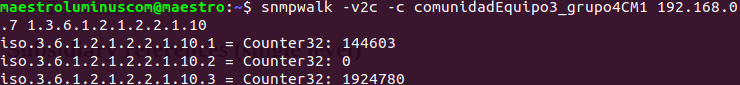
\includegraphics[width=0.8\textwidth]{images/capturas/pregunta4}
	\caption{Consulta SNMP4.}
\end{figure}

\textbf{consulta 5:} Indica cuál interfaz de red ha recibido el mayor número de octetos

\begin{figure}[htbp!]
	\centering
		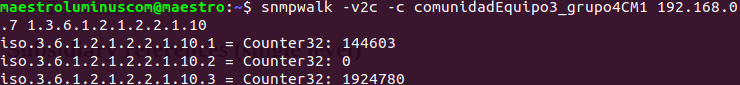
\includegraphics[width=0.8\textwidth]{images/capturas/pregunta5}
	\caption{Consulta SNMP5.}
\end{figure}

\pagebreak
\textbf{consulta 6:} ¿Cuál es la MAC de esa interfaz?

\begin{figure}[htbp!]
	\centering
		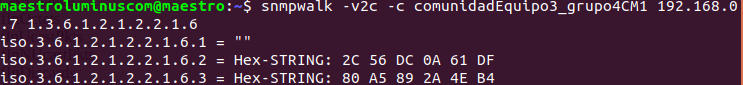
\includegraphics[width=0.8\textwidth]{images/capturas/pregunta6}
	\caption{Consulta SNMP6.}
\end{figure}

\textbf{consulta 7:} ¿Cuántos mensajes ICMP ha recibido el agente?

\begin{figure}[htbp!]
	\centering
		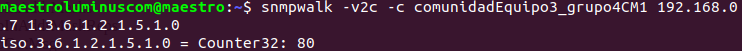
\includegraphics[width=0.8\textwidth]{images/capturas/pregunta7}
	\caption{Consulta SNMP7.}
\end{figure}

\textbf{consulta 8:} ¿Cuántas entradas tiene la tabla de enrutamiento IP?

\begin{figure}[htbp!]
	\centering
		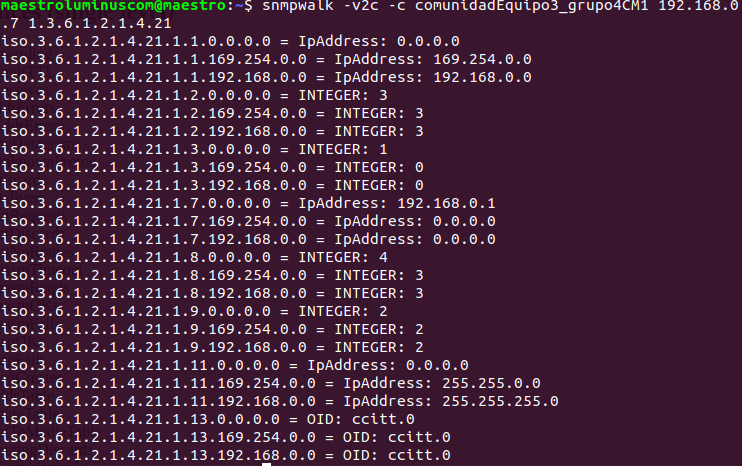
\includegraphics[width=0.8\textwidth]{images/capturas/pregunta8}
	\caption{Consulta SNMP8.}
\end{figure}

\textbf{consulta 9:} ¿Cuántos datagramas UDP ha recibido el agente?

\begin{figure}[htbp!]
	\centering
		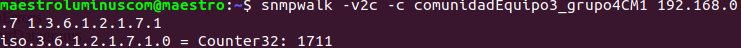
\includegraphics[width=0.8\textwidth]{images/capturas/pregunta9}
	\caption{Consulta SNMP9.}
\end{figure}

\pagebreak
\textbf{consulta 10:} ¿El agente ha recibido mensajes TCP? ¿Cuántos?

\begin{figure}[htbp!]
	\centering
		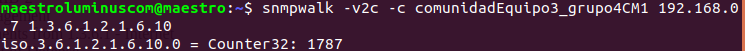
\includegraphics[width=0.8\textwidth]{images/capturas/pregunta10}
	\caption{Consulta SNMP10.}
\end{figure}

\textbf{consulta 11:} ¿Cuántos mensajes EGP ha recibido el agente?

\begin{figure}[htbp!]
	\centering
		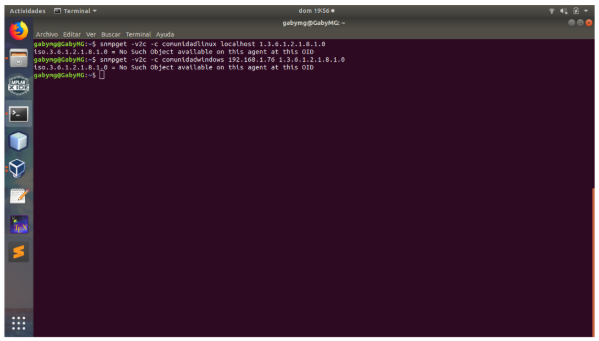
\includegraphics[width=0.8\textwidth]{images/capturas/pregunta11}
	\caption{Consulta SNMP11.}
\end{figure}

\textbf{consulta 12:} Indica el Sistema Operativo que del agente.

\begin{figure}[htbp!]
	\centering
		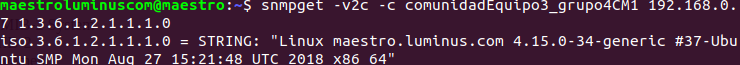
\includegraphics[width=0.8\textwidth]{images/capturas/pregunta12}
	\caption{Consulta SNMP12.}
\end{figure}

\textbf{consulta 13:} Modifica el nombre del contacto o la ubicación del sistema de un agente

\begin{figure}[htbp!]
	\centering
		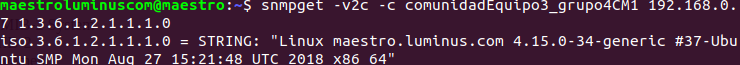
\includegraphics[width=0.8\textwidth]{images/capturas/pregunta12}
	\caption{Consulta SNMP13.}
\end{figure}

\textbf{consulta 14:} Dibuja la MIB del agente.

\begin{figure}[htbp!]
	\centering
		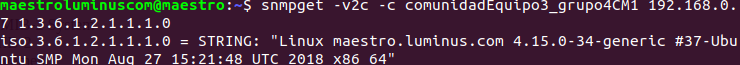
\includegraphics[width=0.8\textwidth]{images/capturas/pregunta12}
	\caption{Consulta SNMP14.}
\end{figure}





